% Unit 060 English translation of chapter4.tex lines 2002--2115.
% Source: Methods of Algebra, Volume 2, commit
% 9a5803ff77dd3257484cb177f851a73770a59dd3 (CC BY 4.0).
% stable-unit-id: o014.aljabr2.chapter4.rlim-homotopy-limit
% Coverage: complete Section 4.10; stops before Section 4.11 at line 2116.

% segment-id: o014.li2.chapter4.rlim-homotopy-limit.h001
\section{Example: \texorpdfstring{$\mathrm{R}\lim$}{Rlim} as a Homotopy Limit}\label{sec:Rlim}
\hypertarget{o014.aljabr2.chapter4.rlim-homotopy-limit}{ }

% segment-id: o014.li2.chapter4.rlim-homotopy-limit.p001
This section continues the discussion of \S\ref{sec:lim1}. Let $\mathcal{A}$
be an abelian category.

% segment-id: o014.li2.chapter4.rlim-homotopy-limit.l001
\begin{lemma}\label{prop:D-countable-product}
	Suppose that $\mathcal{A}$ has exact countable products (respectively,
	exact countable coproducts); see Convention~\ref{con:exact-product}. Then
	every functor in the sequence
	$\cate{C}(\mathcal{A})\to\cate{K}(\mathcal{A})\to\cate{D}(\mathcal{A})$
	preserves countable products (respectively, countable coproducts). In this
	case, there are canonical isomorphisms
	$\Hm^n(\prod_kX_k)\rightiso\prod_k\Hm^n(X_k)$ (respectively,
	$\Hm^n(\bigoplus_kX_k)\rightiso\bigoplus_k\Hm^n(X_k)$).
\end{lemma}
% segment-id: o014.li2.chapter4.rlim-homotopy-limit.pf001
\begin{proof}
	It suffices to prove the product case. Exactness of countable products
	directly gives $\Hm^n(\prod_kX_k)\rightiso\prod_k\Hm^n(X_k)$.

	For every complex $Y$, the definition shows that
	$\Hom^\bullet(Y,\prod_kX_k)$ is isomorphic to the product of the
	$\Hom^\bullet(Y,X_k)$ formed degree by degree in $\cate{C}(\cate{Ab})$.
	Apply exactness of countable products when taking $\Hm^0$ to obtain a
	canonical isomorphism
	$\Hom_{\cate{K}(\mathcal{A})}(Y,\prod_kX_k)\simeq
	\prod_k\Hom_{\cate{K}(\mathcal{A})}(Y,X_k)$. Thus
	$\cate{C}(\mathcal{A})\to\cate{K}(\mathcal{A})$ preserves $\prod_k$.

	We now prove that $\cate{K}(\mathcal{A})\to\cate{D}(\mathcal{A})$
	preserves $\prod_k$; the localization functor $Q$ is suppressed. Suppose we
	are given a family of morphisms $f_k:Y\to X_k$ in
	$\cate{D}(\mathcal{A})$. We wish to prove that there is a unique
	$f\in\Hom_{\cate{D}(\mathcal{A})}(Y,\prod_kX_k)$ satisfying
	$p_hf=f_h$ for every $h$, where $p_h:\prod_kX_k\to X_h$ is the canonical
	projection in $\cate{K}(\mathcal{A})$. We may assume that each $f_k$ is
	represented by a diagram in $\cate{K}(\mathcal{A})$
	\begin{equation}\label{eqn:D-countable-product-aux0}
		Y \xrightarrow{b_k} Z_k \xleftarrow{s_k} X_k, \quad s_k:\; \text{a quasi-isomorphism}.
	\end{equation}
	The morphism $s:=\prod_ks_k:\prod_kX_k\to\prod_kZ_k$ remains a
	quasi-isomorphism. The diagram
	\[ Y \xrightarrow{b := (b_k)_k} \prod_k Z_k \xleftarrow{s} \prod_k X_k \]
	determines $f\in\Hom_{\cate{D}(\mathcal{A})}(Y,\prod_kX_k)$. Notice that
	$f$ depends only on $(f_k)_k$, not on the choices made in
	\eqref{eqn:D-countable-product-aux0}. The commutativity of the following
	diagram implies that $p_hf=f_h$ for every $h$:
% segment-id: o014.li2.chapter4.rlim-homotopy-limit.g001
	\[\begin{tikzcd}
		& Z_h & X_h \arrow[l, "s_h"'] \\
		Y \arrow[r, "b"'] \arrow[ru, "b_h"] & \prod_k Z_k \arrow[u] & \prod_k X_k \arrow[l, "s"] \arrow[u, "p_h"'] .
	\end{tikzcd} \]

	If $g\in\Hom_{\cate{D}(\mathcal{A})}(Y,\prod_kX_k)$ also satisfies
	$p_hg=f_h$ for every $h$, there is a commutative diagram in
	$\cate{K}(\mathcal{A})$
% segment-id: o014.li2.chapter4.rlim-homotopy-limit.g002
	\[\begin{tikzcd}
		& M_h & X_h \arrow[l, "t_h"'] \\
		Y \arrow[r, "c"] \arrow[ru, "c_h"] \arrow[rd, "{(c_k)_k}"'] & M \arrow[u, "r_h"'] \arrow[d, "(r_k)_k"] & \prod_k X_k \arrow[l, "t"'] \arrow[u, "p_h"'] \arrow[ld, "u"] \\
		& \prod_k M_k &
	\end{tikzcd} \quad \begin{array}{l}
		h \in \Z, \\
		t, t_h:\;\text{quasi-isomorphisms}, \\
		u := (r_k)_k t = \prod_k t_k ,
	\end{array}\]
	such that the second row represents $g$, while the
	$\begin{tikzpicture}[xscale=0.3, yscale=0.3, baseline=(O)]
		\coordinate (O) at (0, -0.8);
		\draw[->] (0,-1) -- (1, 0) -- (2, 0);
	\end{tikzpicture}$
	part represents $f_h$. The square is constructed using the version of
	condition (S3) in Definition~\ref{def:multiplicative-family} for a right
	multiplicative system, while commutativity of the lower part is immediate.

	Exactness of $\prod_k$ shows that $u$ is a quasi-isomorphism. Consequently,
	$g$ is also represented by the
	$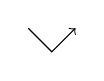
\begin{tikzpicture}[xscale=0.3, yscale=0.3, baseline=(O)]
		\coordinate (O) at (0, -0.8);
		\draw[->] (0,0) -- (1, -1) -- (2, 0);
	\end{tikzpicture}$
	part of the diagram. But $Y\xrightarrow{c_k}M_k\xleftarrow{t_k}X_k$
	represents $f_k$. Comparing this with the construction of $f$ above gives
	$f=g$.
\end{proof}

% segment-id: o014.li2.chapter4.rlim-homotopy-limit.r001
\begin{remark}
	If the indexing set for the product (respectively, coproduct) is replaced by
	an arbitrary small set $I$, the corresponding statement remains valid.
\end{remark}

% segment-id: o014.li2.chapter4.rlim-homotopy-limit.p002
Let $\mathcal{D}$ be an $\cate{Ab}$-category. Consider the category
$\cate{InvSys}(\mathcal{D}):=\mathcal{D}^{\Z_{\geq0}^{\opp}}$ from
\eqref{eqn:InvSys}. Its objects are data $X=(X_k,f_k)_{k\geq0}$, where
$X_k\in\Obj(\mathcal{D})$ and
$f_k\in\Hom_{\mathcal{D}}(X_{k+1},X_k)$. If $\mathcal{D}$ has countable
products, define the canonical morphism as in
Definition~\ref{def:Delta-diff}:
	\[ \Delta_X := T_X - \identity: \prod_k X_k \to \prod_k X_k. \]
\index[sym1]{InvSys}
\index[sym1]{DirSys@$\cate{DirSys}$}

% segment-id: o014.li2.chapter4.rlim-homotopy-limit.p003
Dually, an object of the category
$\cate{DirSys}(\mathcal{D}):=\mathcal{D}^{\Z_{\geq0}}$ consists of data
$X=(X_k,g_k)_{k\geq0}$\footnote{Such data are also called a direct system in
$\mathcal{D}$.}, where $X_k\in\Obj(\mathcal{D})$ and
$g_k\in\Hom_{\mathcal{D}}(X_k,X_{k+1})$. Similarly, define
$\nabla_X:=T_X-\identity:\bigoplus_kX_k\to\bigoplus_kX_k$, assuming that
$\mathcal{D}$ has countable coproducts; $T_X$ is again the analogous shift
morphism.

% segment-id: o014.li2.chapter4.rlim-homotopy-limit.p004
If $\Ker(\Delta_X)$ or $\Coker(\nabla_X)$ exists, there are canonical
isomorphisms
\begin{align*}
	X \in \Obj\left( \cate{InvSys}(\mathcal{D}) \right) & \implies \varprojlim_k X_k \simeq \Ker(\Delta_X), \\
	X \in \Obj\left( \cate{DirSys}(\mathcal{D}) \right) & \implies \varinjlim_k X_k \simeq \Coker(\nabla_X).
\end{align*}
The naive hope is to apply this to $\mathcal{D}=\cate{D}(\mathcal{A})$.
Derived categories are rarely abelian categories. Nevertheless,
Remark~\ref{rem:homotopy-kernel-cokernel} shows that mapping cones can serve as
homotopical versions of kernels and cokernels. Roughly speaking, the analogous
construction in a triangulated category is a distinguished triangle.

% segment-id: o014.li2.chapter4.rlim-homotopy-limit.d001
\begin{definition}[M.\ Bökstedt, A.\ Neeman {\cite{BN93}}]\label{def:holim}
	\index{homotopy limit, homotopy colimit}
	\index[sym1]{holim@$\holim$, $\hocolim$}
	Let $\mathcal{D}$ be a triangulated category.
	\begin{itemize}
		\item If $\mathcal{D}$ has countable products, a \emph{homotopy limit}
		(or homotopy $\varprojlim$) of an object
		$X\in\Obj(\cate{InvSys}(\mathcal{D}))$ means a distinguished triangle
		\[ \holim(X) \to \prod_k X_k \xrightarrow{\Delta_X} \prod_k X_k \xrightarrow{+1} . \]
		\item If $\mathcal{D}$ has countable coproducts, a \emph{homotopy
		colimit} (or homotopy $\varinjlim$) of an object
		$X\in\Obj(\cate{DirSys}(\mathcal{D}))$ means a distinguished triangle
		\[ \bigoplus_k X_k \xrightarrow{\nabla_X} \bigoplus_k X_k \to \hocolim(X) \xrightarrow{+1} . \]
	\end{itemize}
\end{definition}

% segment-id: o014.li2.chapter4.rlim-homotopy-limit.p005
The distinguished triangles occurring in this definition are isomorphic to
one another (Corollary~\ref{prop:Cone-uniqueness}), but the isomorphisms are
not canonical.

% segment-id: o014.li2.chapter4.rlim-homotopy-limit.p006
Return to complexes. Observe that
$\cate{InvSys}(\cate{C}(\mathcal{A}))=
\cate{C}(\cate{InvSys}(\mathcal{A}))$; the objects of both categories are the
same commutative diagrams
% segment-id: o014.li2.chapter4.rlim-homotopy-limit.g003
\[\begin{tikzcd}
	& \vdots \arrow[d, "{f_1^n}"'] & \vdots \arrow[d, "{f_1^{n+1}}"] & \\
	\cdots \arrow[r] & X_1^n \arrow[r, "{d_{X_1}^n}"] \arrow[d, "{f_0^n}"'] & X_1^{n+1} \arrow[d, "{f_0^{n+1}}"] \arrow[r] & \cdots \\
	\cdots \arrow[r] & X_0^n \arrow[r, "{d_{X_0}^n}"] & X_0^{n+1} \arrow[r] & \cdots
\end{tikzcd} \quad \text{with each row a complex}. \]
Morphisms in the two categories are likewise the same two-level commutative
diagrams. Thus, in $\mathcal{D}:=\cate{D}(\mathcal{A})$, we can compare
$\holim(X)$ with the right derived functor $\mathrm{R}\lim(X)$ of
$\varprojlim$, provided that both exist.

% segment-id: o014.li2.chapter4.rlim-homotopy-limit.p007
Also observe that the cohomology $\Hm^m$ of an object
$X\in\cate{C}(\cate{InvSys}(\mathcal{A}))$ is
$(\Hm^m(X_k),\Hm^m(f_k))_{k\geq0}$. Thus $X\to Y$ is a quasi-isomorphism if
and only if every $X_k\to Y_k$ is a quasi-isomorphism in
$\cate{C}(\mathcal{A})$.

% segment-id: o014.li2.chapter4.rlim-homotopy-limit.t001
\begin{theorem}\label{prop:Rlim-as-holim}
	Suppose that $\mathcal{A}$ is an abelian category with exact countable
	products and enough injective objects.
	\begin{enumerate}[(i)]
		\item The right derived functor of the left-exact functor
		$\varprojlim:\cate{InvSys}(\mathcal{A})\to\mathcal{A}$ exists and is
		written
		\[ \mathrm{R}\lim :  \cate{D}^+\left(\cate{InvSys}(\mathcal{A})\right) \to \cate{D}^+(\mathcal{A}) . \]
		\item For every object $X=(X_k,f_k)_{k\geq0}$ of
		$\cate{C}^+(\cate{InvSys}(\mathcal{A}))$, there is a distinguished
		triangle in $\cate{D}(\mathcal{A})$
		\[ \mathrm{R}\lim(X) \to \prod_k X_k \xrightarrow{\Delta_X} \prod_k X_k \xrightarrow{+1}. \]
		In particular, $\mathrm{R}\lim(X)\simeq\holim(X)$.
		\item The dimension of $\mathrm{R}\lim$ in the sense of
		Definition--Proposition~\ref{def:dim-functor} is at most $1$.
	\end{enumerate}
\end{theorem}
% segment-id: o014.li2.chapter4.rlim-homotopy-limit.pf002
\begin{proof}
	Since $\cate{InvSys}(\mathcal{A})$ has enough injective objects, (i) holds.
	More precisely, take the category $\mathcal{R}$ from
	Lemma~\ref{prop:lim1-prep} and apply
	Theorem~\ref{prop:resolution-existence} to
	$\cate{InvSys}(\mathcal{A})$ and $\mathcal{R}$. For every
	$X=(X_k,f_k)_{k\geq0}$ in
	$\cate{C}^+(\cate{InvSys}(\mathcal{A}))$, there is a quasi-isomorphism
	$X\to Y$ with $Y\in\Obj(\cate{C}^+(\mathcal{R}))$. Then
	$\mathrm{R}\lim(X)=\varprojlim Y$. The definition of $\mathcal{R}$ ensures
	that $\Delta_Y$ is surjective degree by degree, so there is a short exact
	sequence in $\cate{C}^+(\mathcal{A})$
	\[ 0 \to \varprojlim Y \to \prod_{k \geq 0} Y_k \xrightarrow{\Delta_Y} \prod_{k \geq 0} Y_k \to 0. \]
	Furthermore, every $X_k\to Y_k$ is a quasi-isomorphism, so
	$\prod_{k\geq0}X_k\to\prod_{k\geq0}Y_k$ is also a quasi-isomorphism. This
	gives the distinguished triangle in (ii):
	\[ \mathrm{R}\lim(X) \to \prod_{k \geq 0} X_k \xrightarrow{\Delta_X} \prod_{k \geq 0} X_k \xrightarrow{+1} . \]

	For (iii), if $X\in\Obj(\cate{InvSys}(\mathcal{A}))$, then $\Delta_X$ is
	a morphism in $\cate{InvSys}(\mathcal{A})$, and
	$\holim(X)\simeq\Cone(\Delta_X)[-1]$ lies in
	$\Obj(\cate{D}^{[0,1]}(\mathcal{A}))$. This is also a restatement of
	Theorem~\ref{prop:lim1}.
\end{proof}

% segment-id: o014.li2.chapter4.rlim-homotopy-limit.p008
There is a dual version of Theorem~\ref{prop:Rlim-as-holim} for
$\varinjlim:\cate{DirSys}(\mathcal{A})\to\mathcal{A}$; we do not repeat the
details.

% segment-id: o014.li2.chapter4.rlim-homotopy-limit.p009
Example~\ref{eg:Rlim-unbounded} will show how to obtain
$\mathrm{R}\lim$ on the unbounded derived category so that
Theorem~\ref{prop:Rlim-as-holim} (ii) remains valid.
